\renewcommand{\arraystretch}{1.5}
\begin{longtable}{
    |p{4cm}
    |p{3cm}
    |p{3cm}
    |p{3cm}|
}
\caption{Comparativa de sensores para medición de pH.}
\label{tab:sensores_ph} \\
\hline
\textbf{Característica} 
    & \textbf{Gravity: Analog pH Meter V2 \cite{DFRobot_pH_Sensor}} 
    & \textbf{Gravity: Industrial Analog pH Meter Pro Kit V2 \cite{DFRobot_pH_Sensor}} 
    & \textbf{Atlas Scientific EZO-pH™ \cite{AtlasScientific_pH_Kit}} \\ 
\hline
\endfirsthead

\hline
\textbf{Característica} 
    & \textbf{Gravity: Analog pH Meter V2 \cite{DFRobot_pH_Sensor}} 
    & \textbf{Gravity: Industrial Analog pH Meter Pro Kit V2 \cite{DFRobot_pH_Sensor}} 
    & \textbf{Atlas Scientific EZO-pH™ \cite{AtlasScientific_pH_Kit}} \\ 
\hline
\endhead

\hline
\multicolumn{4}{r}{\textit{Continúa en la siguiente página}} \\
\endfoot

\hline
\endlastfoot

Rango de medición 
    & 0--14 pH 
    & 0--14 pH 
    & 0--14 pH \\ \hline

Precisión 
    & $\pm$0.1 pH @ 25°C 
    & $\pm$0.1 pH @ 25°C 
    & $\pm$0.002 pH \\ \hline

Tipo de salida 
    & Analógica (0--3.0 V) 
    & Analógica (0--3.0 V) 
    & UART, I2C, Analógica \\ \hline

Voltaje de operación 
    & 3.3--5.5 V 
    & 3.3--5.5 V 
    & 3.3--5.5 V \\ \hline

Compatibilidad ESP32 
    & Sí (ADC) 
    & Sí (ADC) 
    & Sí (UART/I2C/ADC) \\ \hline

Tipo de sonda 
    & Grado laboratorio 
    & Grado industrial 
    & Grado laboratorio/industrial \\ \hline

Longitud del cable de sonda 
    & 100 cm 
    & 500 cm 
    & 100 cm (extensible) \\ \hline

Diseñado para monitoreo continuo 
    & No 
    & Sí 
    & Sí \\ \hline

Vida útil 
    & $>$0.5 años (Dependiendo frecuencia de uso) 
    & $>$0.5 años (uso 24/7) 
    & $>$2.5 años \\ \hline

Tiempo de respuesta 
    & $<$2 min 
    & $<$1 min 
    & $<$1 min \\ \hline

Costo aproximado 
    & \$39.50 USD 
    & \$64.90 USD 
    & \$159.99 USD \\ \hline

Ventajas 
    & Económico, fácil de usar 
    & Resistente, ideal para ambientes hostiles 
    & Alta precisión, múltiples interfaces de comunicación \\ \hline

Desventajas 
    & No apto para uso continuo 
    & Mayor costo que versión V2 
    & Muy costoso y compleja integración \\ \hline

Imagen
    & \shortstack{\\ 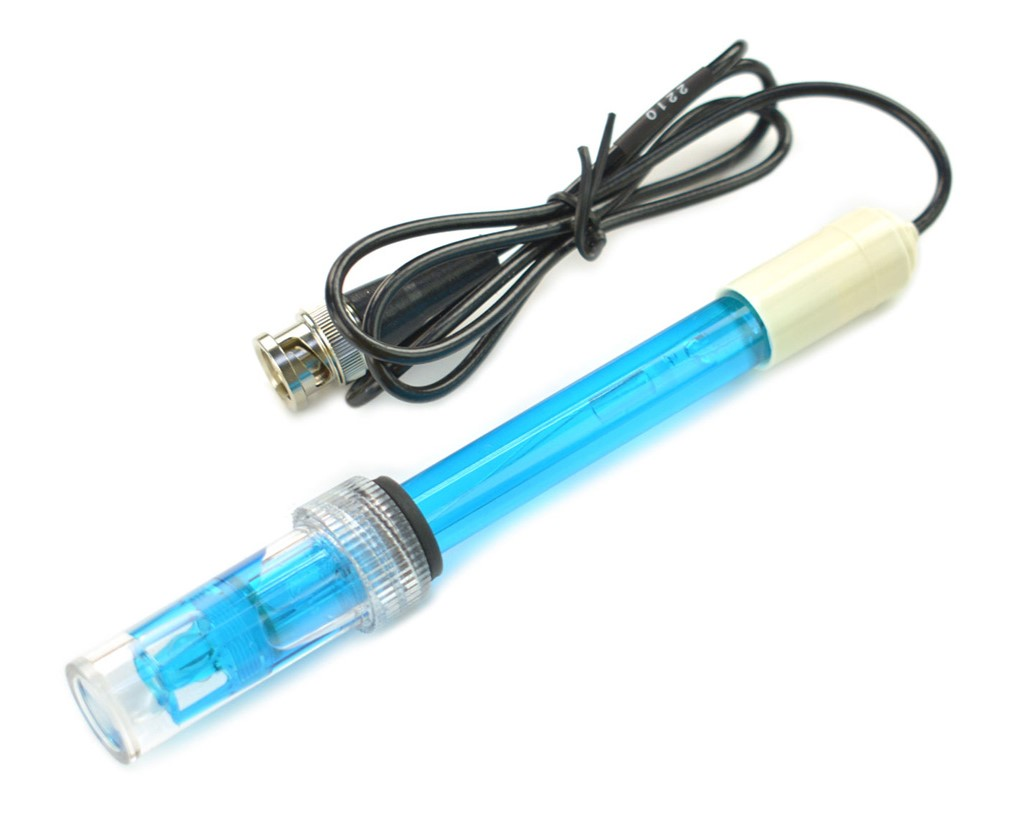
\includegraphics[width=1\linewidth]{Documento/Imagenes/Análisis/sensores/pH_sensor.jpg}}
    & \shortstack{\\ 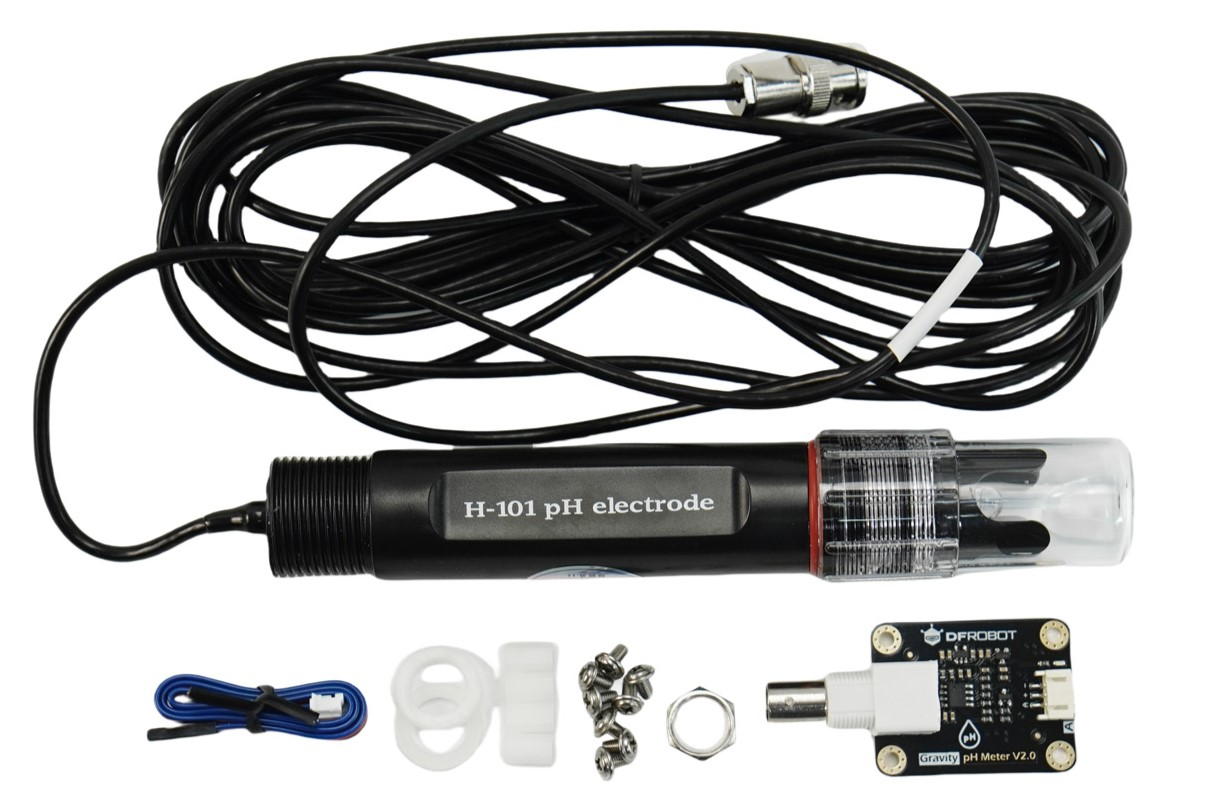
\includegraphics[width=1\linewidth]{Documento/Imagenes/Análisis/sensores/pH pro sensor.jpg}}
    & \shortstack{\\ 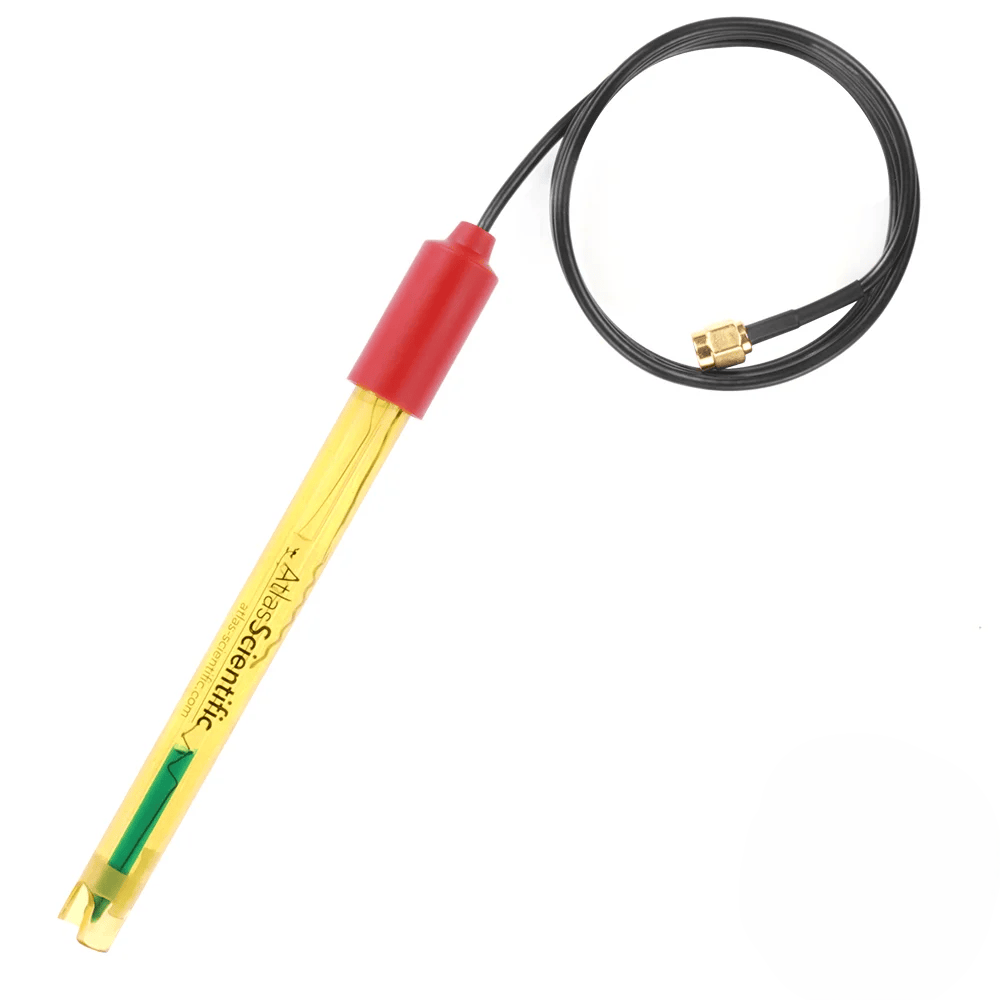
\includegraphics[width=1\linewidth]{Documento/Imagenes/Análisis/sensores/ph atlas sensor.png}} \\ \hline

\end{longtable}
